\documentclass[NormeDiProgetto.tex]{subfiles}

\begin{document}
	\chapter{Processi organizzativi}

	\section{Processi di cordinamento}
	
	\subsection{Comunicazione}
	In questa sezione vengono illustrate le norme che regolano la comunicazione sia tra i membri del gruppo 353 che con entità esterne, come i Committenti e i Proponenti.
	\subsubsection{Comunicazioni interne}
	Le comunicazioni interne al gruppo vengono effettuate tramite \citaGloss{Slack}, un'applicazione di messaggistica multi piattaforma con funzionalità specifiche per gruppi di lavoro. La decisione di utilizzare questo strumento è stata supportata dalle funzionalità di integrazione di \citGloss{Bot} e di creazione di canali tematici, utili per poter classificare le conversazioni e permettere una comunicazione più efficace e mirata. 
	\\
	Inoltre è stato deciso di affiancare \citGloss{Skype} per effettuare video chiamate in caso di impossibilità di riunirsi personalmente. \'{E} stato scelto questo metodo poiché immediato e di facile utilizzo.
	\\
	All'interno di \citGloss{Slack} sono stati predisposti dei canali tematici, suddivisi per argomento in questo modo:
	\begin{itemize}
		\item \textbf{general}: Per discutere tutto ciò che riguarda l'organizzazione generale del progetto, la scelta degli strumenti di lavoro e per prendere decisioni in modo rapido. Inoltre qui vengono decisi gli argomenti principali da discutere nelle riunioni;
		\item \textbf{calendario\underline{ }meeting}: Il canale riservato nel quale un \citGloss{Bot} notifica giornalmente gli eventi facenti parte del calendario comune, come riunioni interne, eventi di formazione o riunioni esterne;
		\item \textbf{daily\underline{ }standup}: Il canale dedicato a un \citGloss{Bot} che giornalmente chiede ai partecipanti notizie sulle attività svolte nel giorno precedente e quelle che sono programmate per il giorno corrente. Inoltre viene chiesto se si sono verificati problemi nelle attività in corso, così da aiutare il gruppo a organizzarsi e a concentrare gli sforzi su particolari attività;
		\item \textbf{github\underline{ }notifications}: Il canale creato affinché un \citGloss{Bot} invii una notifica ogni qualvolta un membro del gruppo effettua un operazione su Github;
		\item \textbf{random}: Un canale generico, dove il gruppo discute liberamente di questioni non riguardanti il progetto e il suo sviluppo.
		
	\end{itemize}
	Sono stati creati anche dei canali appositi per gestire meglio la stesura dei documenti, nello specifico:
	\begin{itemize}
		\item \textbf{analisi\underline{ }requisiti}: Per commentare i casi d'uso e i requisiti necessari per la stesura del documento \adr;
		\item \textbf{piano\underline{ }progetto}: Per confrontarsi sulla ripartizione dei ruoli e del monte ore a essi associato da includere nel \pdp;
		\item \textbf{piano\underline{ }qualifica}: Per discutere riguardo gli obiettivi e le strategie da applicare per garantire qualità e gestire verifica e validazione.
	\end{itemize}
	
	\subsubsection{Comunicazioni esterne}
	Questa sottosezione raccoglie le norme che regolano le comunicazioni con soggetti esterni al gruppo 353, i quali sono:
	\begin{itemize}
		\item La proponente \textbf{RedBabel} rappresentata da Alessandro Maccagnan e Milo Ertola, con i quali si intende stabilire un rapporto di collaborazione a fine di definire i requisiti che permetteranno la realizzazione del prodotto;
		\item \textbf{Prof. Tullio Vardanega} e \textbf{Prof. Riccardo Cardin}, ai quali verrà fornita la documentazione richiesta in ciascuna revisione di progetto, con i quali si intende dialogare con fine il miglioramento continuo.
	\end{itemize}
	\paragraph{Comunicazioni esterne scritte}
	Le comunicazioni esterne scritte vengono effettuate utilizzando l'indirizzo email del gruppo:
	\begin{center}
		\mailleaf
	\end{center}
	a cui ogni membro del gruppo ha accesso.\\
	Per comunicare con i Proponenti vengono utilizzati gli indirizzi email forniti durante la presentazione dei capitolati, rispettivamente 
	\begin{center}
		\mail{alessandro@redbabel.com} \\
		e\\
		\mail{milo@redbabel.com}
		
	\end{center}
	Inoltre è stato creato in \citGloss{Slack} un canale apposito per comunicare in maniera immediata con i proponenti, per accordarsi riguardo eventuali incontri e specifiche di progetto.\\
	Per comunicare con i Committenti si utilizza l'indirizzo di posta elettronica, utilizzando un oggetto specifico e conciso per descrivere il contenuto del messaggio. Ci si rivolge ai committenti dando loro del Voi o del Lei.
	
	\subsection{Riunioni}
	Questa sotto-sezione definisce le regole che normano le riunioni, interne o esterne, e il loro svolgimento. Durante lo svolgimento di ogni riunione, verrà nominato un segretario tra i membri del gruppo 353, il cui compito verterà nel far rispettare l'ordine del giorno, annotare gli argomenti discussi e redarre il Verbale di Riunione.
	\subsubsection{Verbale di riunione}
	Redigere il Verbale di Riunione è il compito del segretario, il quale sarà strutturato secondo questo scheletro:
	\begin{itemize}
		\item \textbf{Verbale TIPO del DATA:} costituirà il frontespizio;
		\begin{itemize}
			\item \textbf{LUOGO:} indica la tipologia d'incontro ossia se Interno o Esterno;
			\item \textbf{DATA:} indica il giorno in cui si è svolta la riunione mentre per 
		\end{itemize}
		\item \textbf{Informazioni sulla riunione}: questa sezione contiene:
		\begin{itemize}
			\item \textbf{Motivo della riunione}: sotto forma di paragrafo, che illustra i motivi generali della riunione; 
			\item \textbf{Luogo e Data}: ad esempio, Padova 05 Dicembre 2017;
			\item \textbf{Ora di inizio}: nel formato ventiquattro ore, ad esempio 13:15;
			\item \textbf{Ora di fine}: nel formato ventiquattro ore, ad esempio 15:30;
			\item \textbf{Partecipanti}: elencati iniziando da Proponente/Committenti se la riunione è esterna, seguiti dai membri del gruppo partecipanti;
			\end{itemize}
			\item \textbf{Ordine del Giorno}: indicato come elenco puntato degli argomenti da discutere;
			\item \textbf{Resoconto}: contiene il riassunto redatto dal segretario secondo i punti dell'ordine del giorno, precisando se sono stati discussi e le loro relative discussioni.

	\end{itemize}
	\paragraph{Nomenclatura e Conservazione:} i file relativi ai verbali dovranno essere nominati come: \textbf{VER-DATA}.\\
	Ad esempio VER-2017-12-05, per permettere una facile organizzazione dei documenti.
	Essendo documenti ufficiali, devono essere redatti in \LaTeX e inclusi nella \citGloss{repository} omonima.
	
	\subsubsection{Riunioni interne}
	La partecipazione alle riunioni interne è permessa ai soli membri del gruppo 353.
	Il \respdiprog{} ha il compito di stilare l'ordine del giorno, fissare la data e inserirla nel calendario e approvare il verbale redatto dal Segretario.\\
	Di contro, i \textbf{partecipanti} devono presentarsi puntualmente alle riunioni, comunicare eventuali ritardi e partecipare attivamente alle discussioni.\\
	Affinché una riunione sia ritenuta valida, devono essere presenti almeno cinque membri del gruppo 353.
	\subsubsection{Riunioni esterne}
	Le riunioni esterne vedono coinvolti sia i membri del gruppo 353 che alcuni soggetti esterni.\\
	Principalmente le riunioni esterne vengono svolte in Torre Tullio Levi Civita, previa disponibilità dei locali.\\
	A causa della locazione europea dell'azienda proponente, le riunioni verranno effettuate tramite \citGloss{Skype}, per ovviare così al problema della distanza fisica.
	
	\section{Processi di pianificazione}
	\subsection{Ruoli di progetto}
	La realizzazione del progetto è il risultato di un'attività collaborativa tra i membri del gruppo. Ad ogni persona infatti sarà attributo un ruolo, corrispondente a una figura aziendale, per un certo periodo di tempo. A rotazione, ogni membro del gruppo ricoprirà tutti i ruoli di seguito elencati:
	\begin{itemize}
		\item \textbf{Responsabile di progetto};
		\item \textbf{Amministratore};
		\item \textbf{Analista};
		\item \textbf{Progettista};
		\item \textbf{Programmatore};
		\item \textbf{Verificatore}.
	\end{itemize}
	Il cambio del ruolo sarà effettuato in modo da garantire continuità alle attività in corso e far sì che ognuno ricopra ogni ruolo per un tempo omogeneo.\\ L'assegnazione dei ruoli verrà effettuata in modo da non creare condizioni contraddittorie, come ad esempio essere verificatori di documenti prodotti da se stessi, in modo da non compromettere la qualità del lavoro effettuato.
	Spetterà al verificatore il compito di individuare possibili accavallamenti di ruoli.  
	\subsubsection{Responsabile di progetto}
	Il \respdiprog, o "Project Manager", è il responsabile ultimo, per conto del suo gruppo, dei risultati del progetto. Partecipa al progetto per tutta la sua durata e accentra le responsabilità di scelta e di approvazione. Inoltre rappresenta il gruppo di lavoro nei confronti dei Committenti e dei Proponenti. Egli:
	\begin{itemize}
		\item Elabora ed emana piani e scadenze;
		\item Approva l'emissione di documenti;
		\item Coordina le attività del gruppo;
		\item Si relaziona con il controllo di qualità interno al progetto;
		\item Approva l'Offerta e i relativi allegati.
	\end{itemize}

	\subsubsection{Amministratore}
	La figura dell'amministratore è indispensabile per permettere una buona produttività ed efficienza del gruppo, fornendo gli strumenti per adempiere ai propri compiti in maniera regolamentata. Deve gestire l'ambiente di lavoro redigendo i documenti che normano l'attività lavorativa e la loro verifica. Infatti:
	\begin{itemize}
		\item È responsabile della redazione e attuazione di piani e procedure di Gestione per la Qualità;
		\item Controlla il versionamento e le configurazioni dei prodotti;
		\item Collabora alla redazione del \pdp;
		\item Redige le Norme di Progetto;
		\item Si assicura che la documentazione sia corretta, verificata, approvata e facilmente accessibile.
	\end{itemize}

	\subsubsection{Analista}
	L'attività dell'Analista è necessaria e fondamentale affinché il progetto possa essere realizzato. Il suo compito è quello di analizzare il dominio del problema per comprenderlo a pieno, abbassando le probabilità che vengano effettuati gravi problemi di progettazione. I suoi compiti comprendono:
	\begin{itemize}
		\item Lo studio e la definizione del problema da risolvere, per capire cosa deve essere realizzato e definire quindi gli accordi contrattuali in base ai requisiti richiesti;
		\item La verifica delle implicazioni di costo e qualità;
		\item La modellazione concettuale del sistema e la ripartizione dei requisiti;
		\item La realizzazione dello Studio di Fattibilità e dell'Analisi dei Requisiti.
	\end{itemize}
	\subsubsection{Progettista}
	Il Progettista è responsabile delle attività di progettazione, cioè della definizione di una soluzione soddisfacente per tutti gli stakeholder. Gli obiettivi del Progettista comprendono:
	\begin{itemize}
		\item La soddisfazione dei requisiti con un sistema di qualità;
		\item La definizione dell'architettura logica del prodotto in modo che sia facile da mantenere, applicando soluzioni note e ottimizzate;
		\item La suddivisione del sistema in parti di complessità trattabile, per rendere il lavoro di codifica facilmente realizzabile e verificabile;
	\end{itemize} 

	\subsubsection{Programmatore}
	Il programmatore è responsabile delle attività di codifica che portano alla realizzazione del prodotto. Affinché questo avvenga, il suo compito consta solamente di implementare l'architettura definita dal Progettista. Per fare ciò:
	\begin{itemize}
		\item Scrive codice documentato, versionato e manutenibile secondo norme fissate;
		\item Crea le componenti necessarie alla verifica e alla validazione del codice;
		\item Si occupa della stesura del Manuale Utente.
	\end{itemize}

	\subsubsection{Verificatore}
	Il Verificatore è una figura presente per tutta la durata del progetto. Il compito principale è quello di responsabile delle attività di verifica, che comprendono:
	\begin{itemize}
	\item L'accertamento che l'esecuzione delle attività di processo non abbia introdotto errori;
	\item La redazione del \pdq{} che illustra l'esito e la completezza delle verifiche e delle prove effettuate secondo il piano.
	\end{itemize}
	
	\subsubsection{Rotazione dei ruoli}
	Ogni membro del gruppo dovrà ricoprire ciascuno dei ruoli del progetto.\\
	La pianificazione dovrà essere eseguita con precisione rispettando le seguenti regole:
	\begin{itemize}
		\item ogni membro del gruppo non dovrà mai ricoprire un ruolo che preveda la verifica dell'operato svolto da lui in precedenza poiché questo potrebbe	portare ad un conflitto di interesse;
		\item bisogna tener conto dei possibili impegni o interessi dei singoli membri del gruppo;
		\item ogni ruolo, prevedendo comportamenti e attività differenti, dovrà essere trasferito tra i vari membri in modo ottimale lasciando quindi scritto su un documento informale una lista di consigli, procedure da parte dell'ultimo assegnatario di quel ruolo;
		\item ciascun membro dovrà assicurare l’esclusivo svolgimento del ruolo a lui assegnato.
	\end{itemize}
	
	
	\subsection{Ticketing}
	\subsubsection{Task list}
	Il \pdp{} prevede la suddivisione del modello di sviluppo in varie fasi.
	L'insieme delle attività da svolgere in una fase è contenuto in una task list.\\
	Il \respdiprog{} deve realizzare le task list per ogni fase del modello su Asana.
	Ogni task list viene quindi creata dal Responsabile del progetto avente il nome della fase alla quale si riferisce.
	
	\subsubsection{Task:}
	Ogni task viene creata dal \respdiprog{} oppure da un membro del gruppo. Nel secondo caso è richiesta l'approvazione della task da parte della maggioranza (4) dei rimanenti componenti del gruppo.
	Ogni task è quindi composta da un titolo significativo e due date, la prima d'inizio mentre la seconda di termine previsto.
	
	\subsubsection{Ticket:}
	I ticket rappresentano l'unione di una task ad un membro del gruppo.
	L'assegnazione del ticket ad uno specifico componente del gruppo può avvenire secondo due modalità:
	\begin{itemize}
		\item \textbf{Pro-attivamente:} l'assegnatario del task è già noto al momento della creazione dello stesso. In questo caso il ticket viene assegnato direttamente allo specifico componente del gruppo da parte del \respdiprog; 
		\item \textbf{Retroattivamente:} nel caso di task a bassa priorità oppure di grandi quantità di lavoro da parte di tutti i componenti del gruppo, può non essere possibile assegnare direttamente un task ad un componente del gruppo. Questi tasks possono essere auto-assegnati qualora il componente finisse in anticipo i ticket a lui già assegnati.
	\end{itemize}
	
	\section{Procedure}
	\subsection{Creazione e gestione dei task}	
	La procedura di creazione di un task è la seguente:
	\begin{itemize}
		\item accesso alla task list legata alla fase nella quale si vuole che l'attività sia svolta;
		\item creazione del nuovo task;
		\item se il task viene reputato troppo laborioso per essere eseguito individualmente il \respdiprog{} può suddividerlo in sotto-task assegnate a loro volta singolarmente ai membri del gruppo.	
	\end{itemize}		
	
	\subsection{Gestione dei ticket}
	 Ogni ticket si rifà al seguente ciclo di vita a partire dalla sua creazione fino al completamento.\\
	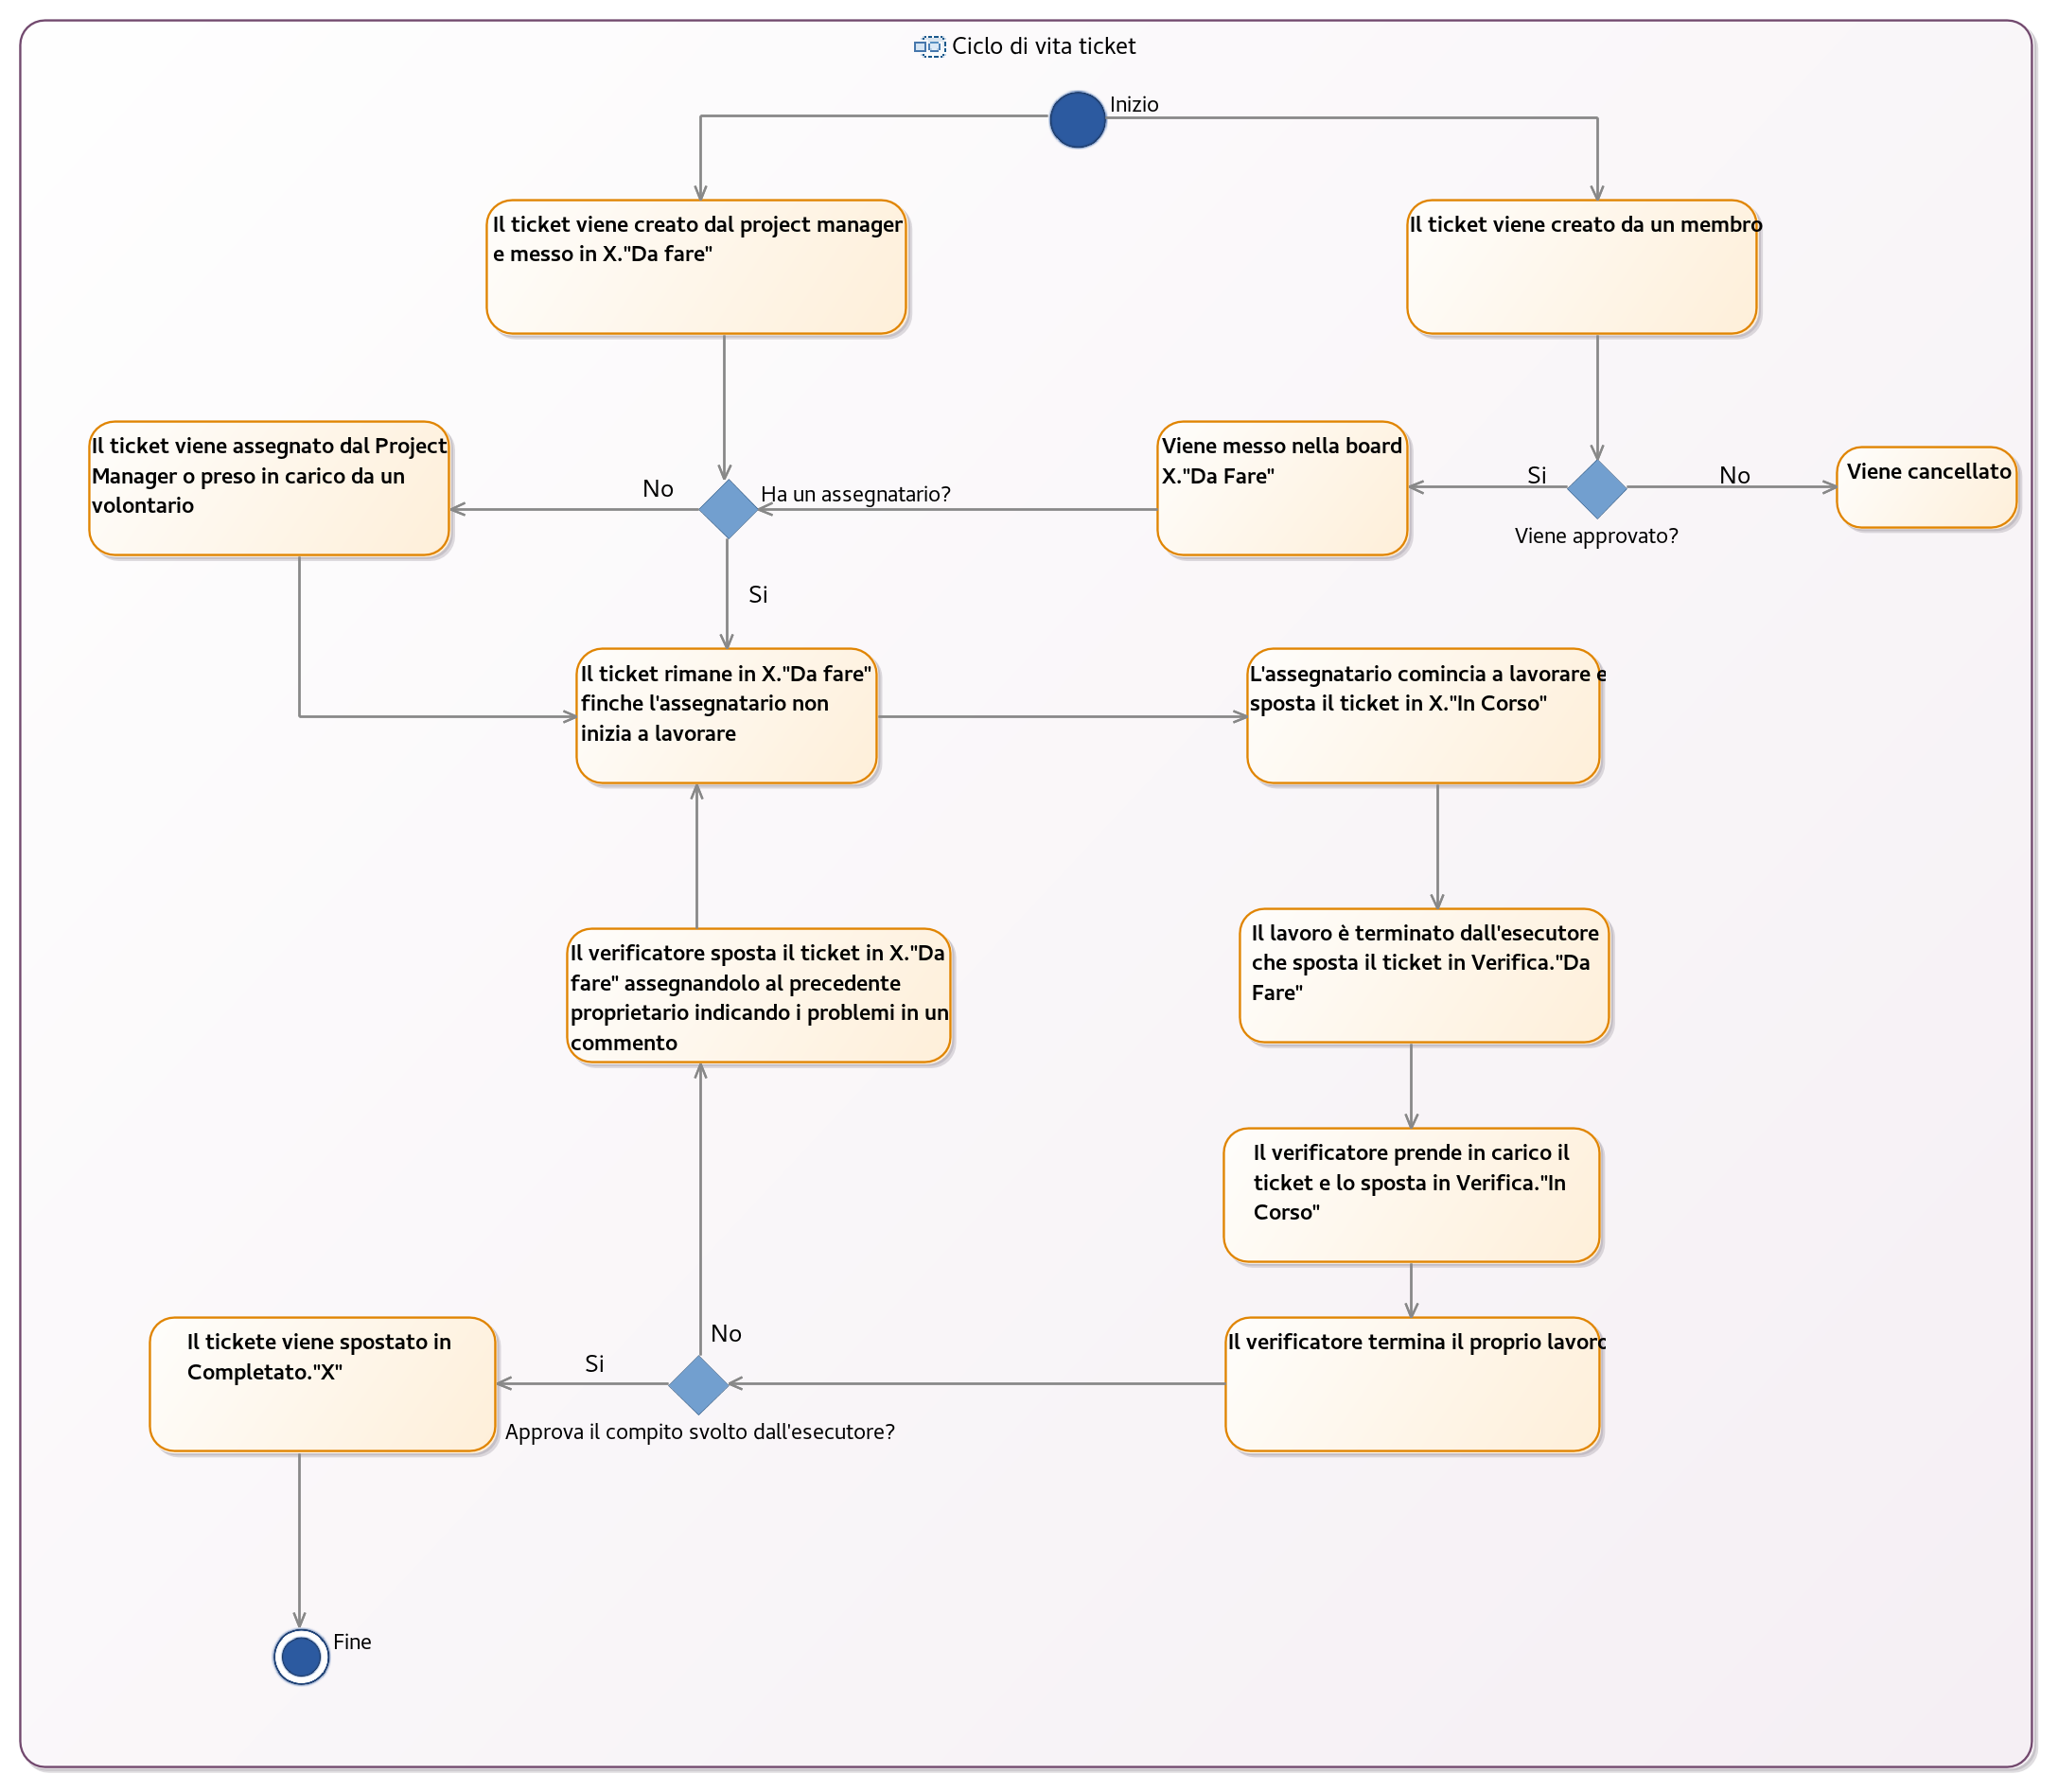
\includegraphics[scale=0.3]{../../common/images/AsanaFlow}
	
	\subsection{Stesura del consuntivo}
	L’operazione di stesura del consuntivo può essere effettuata solamente dal \respdiprog{} della fase corrente.
	Le operazioni che il \respdiprog{} esegue sono le seguenti:
	\begin{enumerate}
		\item  esporta da \citGloss{Asana} tramite \citGloss{Instagantt} un foglio di calcolo, in formato Microsoft Excel, che mostra le ore rendicontate nella fase corrente;
		\item inserisce nel foglio di calcolo precompilato relativo alla fase corrente, realizzato sulla base template disponibile su GitHub;
		\item Inserisce le ore rendicontate nelle celle previste contenete il preventivo delle ore della fase corrente, ottenendo quindi la differenza di ore tra il preventivo e le ore rendicontate;
		\item aggiunge all'interno del \pdp{} una sezione mostrante i valori ottenuti da questo confronto;
		\item crea un a tabella nella sezione descritta punto precedente mostrante la differenza tra le ore preventivate e quelle rendicontate e il budget preventivato rispetto a quello ottenuto dalle ore rendicontate;
		\item trae infine delle conclusioni dai risultati avuti e scrive una valutazione complessiva	del lavoro effettuato nella fase corrente.
	\end{enumerate}
	Per la revisione RR sono effettuati solamente i passaggi dall' 1 al 3 senza effettuare le differenze non avendo ore rendicontate per le fasi successive. Successivamente ad ogni revisione sarà aggiornato il \pdp{} con i valori ottenuti dal confronto tra ore preventivate e rendicontate. 
	
	\section{Strumenti}	
	\subsection{Pianificazione} Per quanto riguarda la pianificazione, la scelta del gruppo 353 è ricaduta sul Asana, strumento per la creazione di task e l'assegnazione delle task con data di inizio e fine per la pianificazione personale del lavoro da svolgere.\\
	Inoltre è possibile:
	\begin{itemize}
		\item creare dipendenze tra attività;
		\item creazione di attività e sotto-attività assegnabili ai membri del progetto
	\end{itemize}

	\subparagraph{Standups:} per incentivare la continuità nel tempo dello sviluppo della commessa, si è scelto di utilizzare Standup Alice, un \citGloss{Bot} per \emph{Slack} per la realizzazione giornaliera di \citGloss{standups}, permettendo al gruppo di seguire costantemente l'operato degli altri componenti e di confrontarsi nel caso sorgano dubbi o domande.
	\subsection{Creazione diagrammi di Gantt}
	Lo strumento scelto per	la realizzazione dei diagrammi di \citGloss{Gant} è GanttProject essendo gratuito, opensource e multi piattaforma.
	\subsection{Calcolo del consuntivo}
	Gli strumenti utilizzati dal \respdiprog{} sono i seguenti:
	\begin{itemize}
		\item \textbf{Instagantt};
		\item \textbf{Libreoffice Calc o Microsoft Excel}.
	\end{itemize}
	
	\section{Formazione}
	\subsection{Formazione dei membri del gruppo}
		La formazione del personale è da realizzarsi in maniera autonoma. I membri del gruppo 353 sono tenuti a studiare individualmente le tecnologie che verranno utilizzate nel corso del progetto. \'{E} possibile che i membri del gruppo realizzino, in piena libertà, delle guide a carattere informale e relative ad un singolo argomento, allo scopo di facilitare la formazione ai restanti componenti del gruppo.
		
	\subsubsection{Ore rendicontabili e di investimento}
	Per distinguere se le ore svolte sono a carico del proponente (rendicontabili) e non di formazione personale (di investimento), si devono rispettare le seguenti regole:
	\begin{enumerate}
		\item \textbf{Incrementato:} il contenuto documento o software è stato modificato venendo ampliato;
		\item \textbf{Standard:} non si sono studiati nuovi concetti, procedure o strumenti.
	\end{enumerate}

	\subsubsection{Guide e materiale utilizzato}
	 La documentazione di riferimento, oltre che al materiale già citato nella sottosezione \emph{Riferimenti Informativi}, comprende:\\
	\begin{itemize}
		\item Per l'utilizzo di \LaTeX: \nURI{https://www.latex-project.org/} \\
		\item Per l'utilizzo di GitHub: \nURI{https://github.com/}\\
		\item Per l'utilizzo di React: \nURI{https://reactjs.org/}\\
		\item Per l'utilizzo di Redux: \nURI{https://redux.js.org/}\\
		\item Per l'utilizzo di Ethereum: \nURI{https://www.ethereum.org/}\\
		\item Per l'utilizzo di Metamask, \nURI{https://metamask.io/}\\ 
		\item Per l'utilizzo di Solidity: \nURI{https://solidity.readthedocs.io/en/develop/}\\
	\end{itemize}
	Il versionamento dei prodotti servirà anche per apprendere dall'operato
	altrui, in modo da integrare le conoscenze personali migliorando la qualità e
	l'efficienza delle attività.
	
\end{document}